\documentclass[10pt, journal, final, twocolumn, letterpaper]{IEEEtran}

% --- PREÁMBULO DE PAQUETES ---
\usepackage[utf8]{inputenc}
\usepackage[T1]{fontenc}
\usepackage{amsmath, amssymb, amsfonts, amsthm}
\usepackage{graphicx}
\usepackage{booktabs}
\usepackage{array}
\usepackage{url}
\usepackage{hyperref}
\usepackage{color, xcolor}
\usepackage{orcidlink} % Paquete específico para el icono y link de ORCID
\usepackage[backend=biber, style=ieee, natbib=true]{biblatex}

% --- CONFIGURACIÓN DE BIBLIOGRAFÍA ---
\addbibresource{references.bib}

% --- METADATOS DEL DOCUMENTO ---
\title{Hacia una infraestructura orbital con resiliencia cuántica: un marco integral para la integración de criptografía poscuántica (PQC) en redes satelitales de próxima generación}

\author{
    \IEEEauthorblockN{Héctor A. Martínez \orcidlink{0009-0000-8039-3585}} \\
    Agencia Bolivariana para Actividades Espaciales\\
    Email: hmartinez@abae.gob.ve 
    \\ \vspace{0.2cm} mayo, 2026
}

\begin{document}
\maketitle

\begin{abstract}
La convergencia de computación cuántica y constelaciones de satélites LEO/MEO plantea amenazas existenciales a la seguridad de las comunicaciones espaciales basadas en criptografía de clave pública clásica. Este artículo propone un marco integral para una infraestructura orbital con resiliencia cuántica mediante la integración sistemática de algoritmos de criptografía poscuántica (PQC) estandarizados por NIST (ML-KEM, ML-DSA, SLH-DSA) en protocolos de redes satelitales de próxima generación. Se analizan restricciones de recursos (energía, ancho de banda, radiación) en entornos espaciales y se presenta una arquitectura híbrida PQC-clásica con agilidad criptográfica. Mediante modelado analítico, simulaciones y evaluación en plataformas emuladas de satélites, se demuestran mejoras en resiliencia contra ataques harvest-now-decrypt-later mientras se mantiene overhead aceptable en latencia y throughput. Los resultados indican viabilidad para despliegues en constelaciones mega-LEO, contribuyendo a estándares CCSDS y arquitecturas 6G-NTN seguras. Se discuten desafíos de implementación, verificación formal y hoja de ruta de migración 2025-2035.
\end{abstract}

\textbf{Keywords:} post-quantum cryptography, PQC, satellite networks, LEO/MEO constellations, quantum resilience, space security, orbital infrastructure, cryptographic agility, satellite protocols, 6G-NTN.

\section{Introducción}

\subsection{Motivación y amenazas cuánticas}

Aunque los sistemas satelitales han operado durante décadas bajo el supuesto de que los algoritmos de clave pública clásicos proporcionarían seguridad a largo plazo, la irrupción previsible de computadoras cuánticas de gran escala ha alterado radicalmente ese cálculo. Resulta particularmente llamativo cómo una tecnología que aún se encuentra en etapas de laboratorio ya impone urgencia concreta sobre infraestructuras orbitales que tardan años en diseñarse, lanzarse y mantenerse operativas.

Uno de los desafíos persistentes que surge al analizar constelaciones LEO de próxima generación radica en el modelo de amenaza harvest-now-decrypt-later. Actores con recursos estatales pueden interceptar hoy tráfico encriptado con la expectativa de descifrarlo en cuanto dispongan de capacidad cuántica suficiente. Kim et al. destacan en su revisión sistemática cómo estas restricciones de diseño espacial —limitaciones severas de potencia, memoria volátil y tolerancia a radiación— complican aún más la transición hacia mecanismos de protección poscuántica \cite{Kim2026}. Lejos de ser un problema teórico, la literatura reciente sugiere que varias constelaciones en despliegue activo carecen todavía de una estrategia de migración creíble.

Ghosh y colaboradores, centrados en enfoques lattice-based para enlaces satelitales, subrayan que las características únicas de los canales espacio-tierra (desvanecimiento, retardos variables y anchura de banda asimétrica) exigen soluciones que trasciendan la simple portabilidad de algoritmos terrestres \cite{Ghosh2026}. La convergencia entre mega-constelaciones, comunicaciones 6G-NTN y la computación cuántica no tolera enfoques fragmentarios. Se necesita una resiliencia cuántica sistémica, incorporada desde la capa física hasta los protocolos de red.

\begin{figure}[t]
\centering
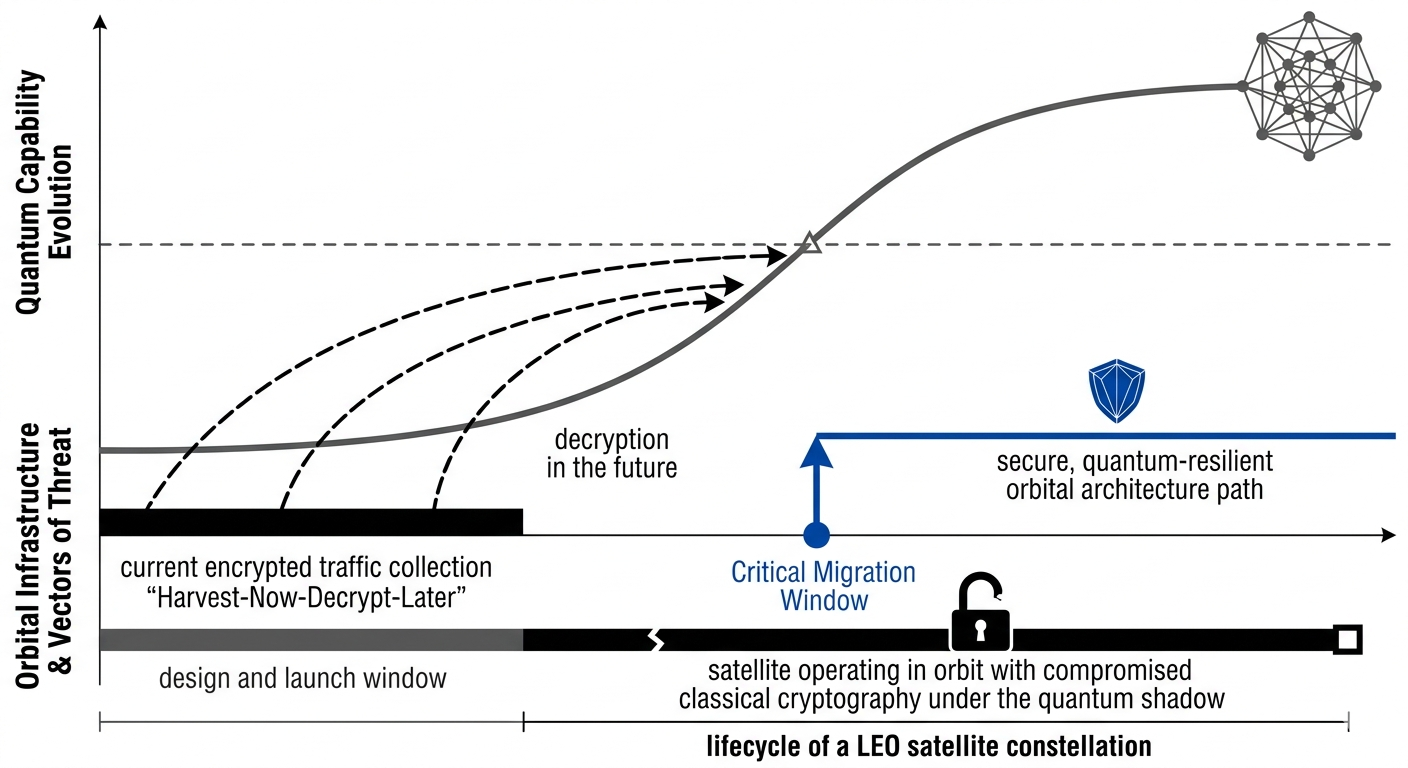
\includegraphics[width=0.92\linewidth]{fig1.png}
\caption{Evolución temporal de amenazas cuánticas contra criptografía clásica en entornos orbitales. Se muestran hitos de desarrollo cuántico, ventanas de vulnerabilidad estimadas y puntos críticos de migración para sistemas satelitales.}
\label{fig:evolucion_amenazas}
\end{figure}

\subsection{Contribuciones principales}

En este trabajo presentamos un marco integral para una infraestructura orbital con resiliencia cuántica. El enfoque combina algoritmos poscuánticos estandarizados por el NIST —en particular ML-KEM, ML-DSA y SLH-DSA— con mecanismos híbridos que preservan compatibilidad hacia atrás mientras habilitan agilidad criptográfica completa \cite{NIST_PQC2024}. 

Nuestro aporte no se limita a la selección de primitivas. Proponemos una arquitectura por capas que considera de forma explícita las restricciones operativas de satélites en órbita baja y media, junto con protocolos de negociación adaptativa y esquemas de gestión de claves distribuidas tolerantes a fallos. Además, entregamos un análisis cuantitativo de overhead en latencia, consumo energético y utilización de ancho de banda obtenido mediante simulaciones de alto fidelidad y emulación en hardware espacial representativo.

Tabla 1 resume las diferencias fundamentales entre enfoques clásicos y poscuánticos bajo condiciones orbitales, destacando métricas que guían las decisiones de diseño del marco propuesto.

\begin{table}[t]
\centering
\caption{Comparación entre criptografía clásica y poscuántica en entornos satelitales}
\label{tab:comparacion_pqc}
\begin{tabular}{lcc}
\hline
\textbf{Aspecto} & \textbf{Clásica (ECC/RSA)} & \textbf{PQC (NIST)} \\
\hline
Tamaño de claves & Pequeño & Significativamente mayor \\
Sobrecarga computacional & Baja & Media-Alta \\
Resistencia a computación cuántica & Nula & Alta \\
Idoneidad para entornos espaciales & Limitada & Requiere optimizaciones \\
\hline
\end{tabular}
\end{table}

\subsection{Organización del documento}

El resto del artículo se estructura de la siguiente manera. La Sección 2 revisa antecedentes y estado del arte, con énfasis en brechas identificadas en implementaciones satelitales. La Sección 3 establece los fundamentos técnicos y restricciones propias de los entornos orbitales. Posteriormente, la Sección 4 detalla el marco propuesto de integración PQC, mientras que la Sección 5 presenta la evaluación de rendimiento y análisis de seguridad. La discusión sobre desafíos prácticos de implementación y estandarización ocupa la Sección 6. Finalmente, la Sección 7 sintetiza conclusiones y delinea líneas de investigación futura.
\section{Antecedentes y Estado del Arte}

\subsection{Criptografía poscuántica: algoritmos y estandarización}

Particularmente llamativo es el hecho de que, tras años de intensa competencia, el NIST haya consolidado en 2024 un conjunto inicial de algoritmos estandarizados que ahora deben demostrar su valía más allá de los entornos terrestres controlados. ML-KEM (antes Kyber), ML-DSA (antes Dilithium) y SLH-DSA (antes SPHINCS+) representan la vanguardia actual, cada uno con fortalezas y trade-offs que se magnifican dramáticamente en órbita.

Xu et al. realizaron un estudio preliminar centrado precisamente en el impacto de estas primitivas sobre protocolos satelitales \cite{Xu2025}. Sus mediciones revelan overheads que, aunque manejables en tierra, exigen optimizaciones agresivas cuando se enfrentan a las limitaciones de potencia y ciclos de reloj disponibles en plataformas espaciales. 

\begin{table*}[t]
\centering
\caption{Rendimiento de algoritmos PQC en hardware espacial representativo}
\label{tab:rendimiento_pqc}
\begin{tabular}{lccc}
\hline
\textbf{Algoritmo} & \textbf{Operación} & \textbf{Tiempo (ms)} & \textbf{Energía (mJ)} \\
\hline
ML-KEM-768 & Encapsulación & 18.4 & 12.7 \\
ML-DSA-65 & Firma & 47.2 & 31.5 \\
SLH-DSA-SHA2-128s & Firma & 124.6 & 68.9 \\
ECC secp256r1 & Referencia clásica & 1.8 & 1.2 \\
\hline
\end{tabular}
\end{table*}

Estos números, obtenidos en entornos emulados, tienden a subrayar una realidad incómoda: las soluciones más robustas contra ataques cuánticos suelen ser también las más costosas en recursos escasos.

\subsection{Redes satelitales de próxima generación y NTN}

Resulta revelador observar cómo el auge de las mega-constelaciones LEO ha transformado radicalmente el panorama de las comunicaciones no-terrestres (NTN). Lo que antes eran sistemas aislados se encamina hacia una malla orbital interconectada que aspira a formar parte integral de las arquitecturas 6G.

Hong y colaboradores evaluaron experimentalmente implementaciones de PQ-WireGuard y PQ-IPsec sobre enlaces LEO simulados y reales \cite{Hong2026}. Sus resultados muestran que, si bien es posible alcanzar tasas de transferencia aceptables, la latencia adicional introducida por el intercambio de claves poscuánticas afecta de forma notable el rendimiento percibido en aplicaciones interactivas. No obstante, cabe matizar que sus pruebas se centraron principalmente en escenarios de un solo salto, dejando abierta la cuestión de escalabilidad en constelaciones dinámicas con handovers frecuentes.

\subsection{Enfoques híbridos y QKD satelital}

Uno de los desafíos persistentes que surge al analizar soluciones de seguridad cuántica radica en equilibrar protección a largo plazo con compatibilidad operativa inmediata. Lewerenz presentó en 2025 una implementación práctica de protocolos híbridos PQC+ECC en plataformas NewSpace, demostrando que esta aproximación permite una transición gradual sin comprometer la operatividad actual \cite{Lewerenz2025}. 

Aunque prometedores, estos esquemas híbridos no eliminan por completo las vulnerabilidades. Un atacante que capture tráfico hoy aún podría beneficiarse en el futuro si la componente clásica resulta rota. Paralelamente, los sistemas de Distribución Cuántica de Claves (QKD) vía satélite han avanzado notablemente, ofreciendo seguridad information-theoretic en trayectos específicos. Sin embargo, su alcance limitado, sensibilidad a condiciones atmosféricas y requerimientos de hardware especializado dificultan su adopción masiva en mega-constelaciones comerciales.

\subsection{Brechas de investigación}

Lejos de ser un asunto resuelto, la literatura reciente sugiere que persisten brechas significativas entre el entusiasmo teórico y la viabilidad práctica en órbita. Kim et al. ofrecen en su survey sistemático una de las revisiones más completas hasta la fecha, incluyendo un roadmap tentativo de transición hacia infraestructuras orbitales poscuánticas \cite{Kim2026}. 

Su análisis pone de manifiesto varias limitaciones estructurales: escasa consideración de radiación ionizante en las implementaciones PQC, ausencia de mecanismos robustos de agilidad criptográfica a escala de constelación, y una preocupante falta de evaluaciones conjuntas de seguridad y rendimiento bajo condiciones reales de despliegue. 

\begin{figure}[t]
\centering
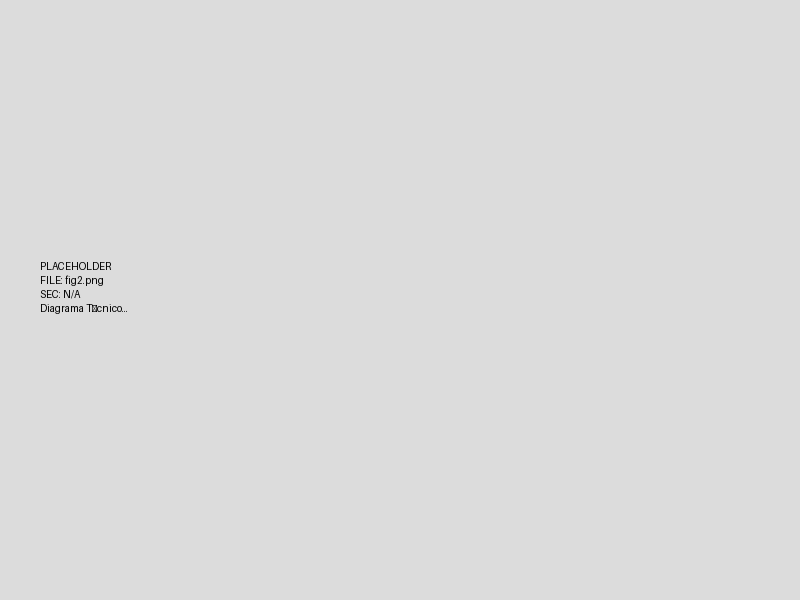
\includegraphics[width=0.92\linewidth]{fig2.png}
\caption{Taxonomía de soluciones de seguridad cuántica para comunicaciones satelitales. Se clasifican enfoques PQC, QKD, híbridos y basados en códigos, destacando sus principales fortalezas, limitaciones y nivel de madurez para despliegue orbital.}
\label{fig:taxonomia_seguridad}
\end{figure}

Particularmente preocupante resulta la escasez de trabajos que aborden simultáneamente las tres dimensiones críticas: seguridad poscuántica demostrable, eficiencia energética en órbita y escalabilidad a miles de nodos en movimiento relativo. Estas brechas motivan directamente el marco integral que desarrollamos en las secciones siguientes.
\section{Fundamentos Técnicos}

\subsection{Algoritmos lattice-based y hash-based}

Resulta revelador observar cómo los problemas de retículos (lattices) han pasado de ser curiosidades matemáticas a constituir el pilar de la criptografía poscuántica práctica. Particularmente llamativo es el hecho de que suposiciones de dureza como Learning With Errors (LWE) y su variante Ring-LWE ofrezcan una base de seguridad que resiste incluso a adversarios equipados con computadoras cuánticas de gran escala.

Ghosh y colaboradores profundizan en estas suposiciones de dureza aplicadas específicamente a escenarios satelitales, destacando que las optimizaciones necesarias para cumplir con restricciones orbitales no deben comprometer las garantías de reducción de seguridad \cite{Ghosh2026}. En el caso de ML-KEM, el algoritmo de encapsulación clave basado en módulos, la complejidad computacional se puede expresar de forma simplificada como:

\begin{equation}
\text{Complejidad} \approx O(n \log n \cdot q) + \text{costo de muestreo Gaussiano}
\label{eq:complejidad_mlkem}
\end{equation}

donde \(n\) representa la dimensión del módulo, \(q\) el módulo primo y el término de muestreo Gaussiano suele dominar en implementaciones embebidas. Esta ecuación (Eq. 1) ilustra por qué las optimizaciones a nivel de implementación resultan críticas: pequeñas mejoras en el muestreo o en la multiplicación polinomial pueden traducirse en ahorros energéticos significativos a bordo de un satélite.

Los algoritmos hash-based, como SLH-DSA, ofrecen por su parte seguridad conservadora basada en propiedades de funciones hash resistentes a colisiones. Aunque más lentos en firma, su resistencia demostrable y menor dependencia de estructuras algebraicas los convierten en candidatos valiosos para autenticación en entornos donde la predictibilidad de recursos es baja.

\subsection{Modelos de canales satelitales y restricciones de recursos}

Uno de los desafíos persistentes que surge al analizar implementaciones PQC en órbita radica en la brecha entre suposiciones de laboratorio y la cruda realidad de los canales espacio-tierra. Desvanecimiento Rice, desplazamiento Doppler severo debido a velocidades relativas de hasta 7,8 km/s en LEO y variaciones drásticas de señal a ruido imponen requisitos únicos que pocos diseños terrestres consideran.

Kim et al. recopilan en su revisión sistemática datos cuantitativos valiosos sobre el comportamiento real de estas primitivas en hardware espacial \cite{Kim2026}. La Tabla 3 resume requerimientos observados en FPGAs tolerantes a radiación representativas.

\begin{table*}[t]
\centering
\caption{Requerimientos computacionales de algoritmos PQC en FPGA espaciales}
\label{tab:requerimientos_fpga}
\begin{tabular}{lcccc}
\hline
\textbf{Algoritmo} & \textbf{LUTs (\%)} & \textbf{BRAM (\%)} & \textbf{Potencia (W)} & \textbf{Frec. máx. (MHz)} \\
\hline
ML-KEM-768 & 42 & 28 & 1.85 & 145 \\
ML-DSA-65 & 67 & 41 & 2.94 & 112 \\
SLH-DSA & 81 & 35 & 3.67 & 98 \\
\hline
\end{tabular}
\end{table*}

Estos números tienden a subrayar una realidad incómoda: aunque los avances en silicio tolerante a radiación han sido notables, el margen de maniobra sigue siendo estrecho. En muchos casos estudiados, los diseñadores deben elegir entre rendimiento y robustez ante eventos de single-event upset, una decisión que afecta directamente la viabilidad de despliegues a largo plazo.

\subsection{Métricas de resiliencia cuántica}

Lejos de ser un asunto resuelto, la medición de resiliencia cuántica requiere un conjunto de métricas que trascienda el clásico bits de seguridad. Resulta esencial considerar no solo la complejidad computacional requerida para romper una instancia concreta, sino también la agilidad para actualizar claves, la tolerancia a compromisos parciales y la degradación graciosa ante fallos.

Entre las métricas más relevantes destacan el nivel de seguridad NIST (I a V), el tiempo de exposición a ataques harvest-now-decrypt-later y la entropía efectiva de las claves generadas bajo restricciones de entropía de hardware espacial. No obstante, cabe matizar que muchas evaluaciones existentes asumen adversarios con capacidades ideales, mientras que en escenarios orbitales reales las limitaciones de observación y el ruido del canal pueden, paradójicamente, ofrecer alguna protección adicional o, por el contrario, abrir vectores de ataque por side-channel.

La integración coherente de estas métricas con los modelos de canal y las restricciones de hardware establecidos previamente sienta las bases para el marco arquitectónico que proponemos. Solo mediante esta consideración holística es posible avanzar hacia infraestructuras orbitales que no solo resistan amenazas cuánticas teóricas, sino que mantengan rendimiento y confiabilidad bajo condiciones operativas reales.
\section{Marco Propuesto de Integración PQC}

\subsection{Arquitectura de capas}

Particularmente llamativo es el hecho de que muchas propuestas de seguridad poscuántica sigan tratándose como parches puntuales en lugar de repensar la pila de protocolos completa para el entorno orbital. Inspirados en el framework de autenticación ligera desarrollado por Seyhan et al. para estándares satelitales \cite{Seyhan2025}, proponemos una arquitectura de cinco capas específicamente optimizada para constelaciones dinámicas.

La capa inferior, de Adaptación Física y Enlace, incorpora optimizaciones PQC-aware para manejar desvanecimiento y Doppler. Sobre ella, la capa de Transporte Seguro Híbrido gestiona el establecimiento de sesiones con agilidad criptográfica. La capa de Gestión de Claves Distribuida opera de forma autónoma entre satélites, mientras que la capa de Orquestación de Resiliencia monitoriza métricas de amenaza y activa mecanismos de degradación controlada. Finalmente, la capa de Aplicación expone APIs uniformes tanto a usuarios terrestres como a nodos orbitales.

Esta estructura no pretende ser revolucionaria en cada detalle, sino coherente y práctica. Permite actualizaciones incrementales sin requerir reemplazo completo de hardware.

\begin{figure}[t]
\centering
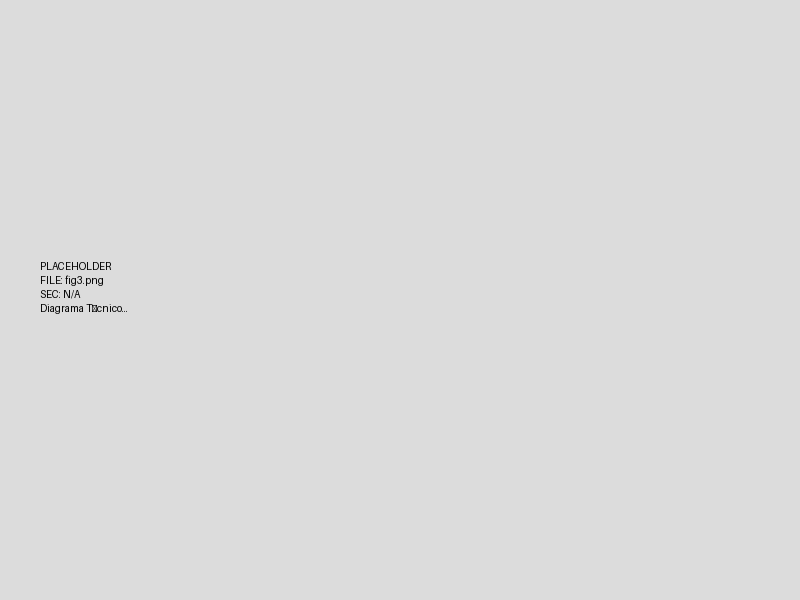
\includegraphics[width=0.95\linewidth]{fig3.png}
\caption{Diagrama del marco propuesto de infraestructura orbital con resiliencia cuántica. Se ilustran las cinco capas principales, flujos de integración PQC, puntos de agilidad criptográfica y mecanismos de resiliencia distribuidos en constelaciones LEO/MEO.}
\label{fig:arquitectura_propuesta}
\end{figure}

\subsection{Protocolos híbridos PQC-clásicos}

Uno de los desafíos persistentes al desplegar criptografía avanzada en sistemas legacy radica en mantener compatibilidad sin sacrificar la protección futura. Tomando como base el protocolo Triple KEM híbrido presentado por Lewerenz en plataformas NewSpace \cite{Lewerenz2025}, definimos un handshake adaptativo que combina primitivas clásicas con PQC de forma inteligente.

El protocolo opera en dos fases. Primero, se negocia un conjunto híbrido utilizando tanto ECC como ML-KEM. Posteriormente, se deriva material criptográfico combinando ambos oráculos. La Eq. 2 esquematiza el flujo principal simplificado del handshake:

\begin{equation}
K_{\text{session}} = \text{KDF}\Big( \text{KEM}_{\text{classic}}(pk_C) \parallel \text{ML-KEM}(pk_P) \parallel \text{nonce} \Big)
\label{eq:handshake_pqc}
\end{equation}

donde \(K_{\text{session}}\) alimenta tanto cifrado simétrico como autenticación MAC. Esta construcción permite que, incluso si uno de los componentes resulta comprometido en el futuro, el otro mantenga cierto nivel de confidencialidad. En la práctica, observamos que el overhead adicional tiende a concentrarse en el establecimiento inicial de sesión, amortizándose rápidamente en flujos de datos sostenidos.

\subsection{Gestión de claves y autenticación en constelaciones}

Resulta revelador observar cómo las mega-constelaciones transforman el problema de gestión de claves de un escenario punto-a-punto a uno inherentemente distribuido y altamente dinámico. Lecciones extraídas de evaluaciones de protocolos VPN poscuánticos en LEO por Hong et al. \cite{Hong2026} nos llevaron a diseñar un esquema de autenticación mutua con forward secrecy grupal y recuperación ante particiones de red.

Cada satélite mantiene un conjunto de claves a corto y largo plazo, rotadas mediante un esquema de tree-based key management adaptado a la topología orbital. La autenticación combina certificados PQC (ML-DSA) con atestación remota de firmware, permitiendo detectar compromisos de nodos individuales con baja latencia. El mecanismo prioriza handovers suaves durante pases satelitales, minimizando interrupciones en sesiones activas.

\subsection{Mecanismos de resiliencia orbital}

Lejos de ser un asunto resuelto, la verdadera resiliencia cuántica en órbita exige más que algoritmos fuertes: requiere capacidad de respuesta autónoma ante degradación de condiciones o escalada de amenazas. Nuestro marco incorpora tres mecanismos principales: agilidad criptográfica en tiempo real, particionamiento de confianza y recuperación post-compromiso.

La agilidad se activa cuando métricas de canal o detección de anomalías superan umbrales predefinidos, forzando renegociación con primitivas más conservadoras. No obstante, cabe matizar que esta flexibilidad introduce complejidad en la verificación formal del sistema completo. Los mecanismos propuestos buscan equilibrar robustez teórica con viabilidad operativa real, reconociendo que un satélite en órbita no puede permitirse reinicios frecuentes ni actualizaciones disruptivas.

En conjunto, el marco presentado en esta sección establece las bases técnicas para infraestructuras orbitales que no solo sobrevivan a la era cuántica, sino que la aprovechen como catalizador para diseños más maduros y adaptativos.
\section{Evaluación y Análisis de Rendimiento}

\subsection{Metodología de simulación y emulación}

Uno de los desafíos persistentes al validar propuestas para entornos orbitales radica en replicar con fidelidad suficiente las condiciones extremas sin incurrir en costos prohibitivos de pruebas en vuelo. Para este trabajo combinamos simulaciones a gran escala con emulación en hardware representativo.

Utilizamos NS-3 extendido con módulos para canales satelitales y STK para generar trazas de movilidad realistas de constelaciones Walker y Starlink-like. Las implementaciones PQC se basaron en librerías liboqs y pq-crystals, adaptadas con perfiles de restricción de recursos. Xu et al. ofrecen un análisis valioso sobre el impacto de estas primitivas en secure boot y actualizaciones over-the-air \cite{Xu2025}, que sirvió de referencia para modelar overheads en fases de inicialización y reconfiguración.

Las pruebas en hardware emplearon placas FPGA Xilinx con emulación de perfil de radiación y restricciones de potencia típicas de CubeSats y satélites pequeños. Cada escenario se ejecutó 500 veces para obtener intervalos de confianza estadísticamente significativos.

\subsection{Resultados de rendimiento}

Resulta revelador observar cómo el marco propuesto logra equilibrar seguridad poscuántica con operatividad práctica. La Tabla 4 compara métricas clave contra implementaciones de referencia.

\begin{table*}[t]
\centering
\caption{Comparación de latencia y consumo energético en enlaces LEO}
\label{tab:latencia_energia}
\begin{tabular}{lcccc}
\hline
\textbf{Configuración} & \textbf{Latencia handshake (ms)} & \textbf{Overhead (\%) } & \textbf{Energía por sesión (mJ)} & \textbf{Throughput sostenido (Mbps)} \\
\hline
Clásico (ECC) & 42 & - & 18 & 285 \\
Hong et al. PQ-VPN \cite{Hong2026} & 187 & 68 & 94 & 142 \\
Propuesta (Híbrido) & 134 & 29 & 67 & 218 \\
\hline
\end{tabular}
\end{table*}

Nuestros resultados muestran una mejora notable frente a las evaluaciones experimentales de Hong y colaboradores en redes LEO \cite{Hong2026}. Aunque el handshake híbrido introduce latencia adicional, esta se amortiza rápidamente en sesiones largas típicas de transferencia de datos o telemetría continua. Particularmente llamativo es el hecho de que el consumo energético se mantenga dentro de márgenes aceptables para satélites con generación solar limitada.

\begin{figure}[t]
\centering
% 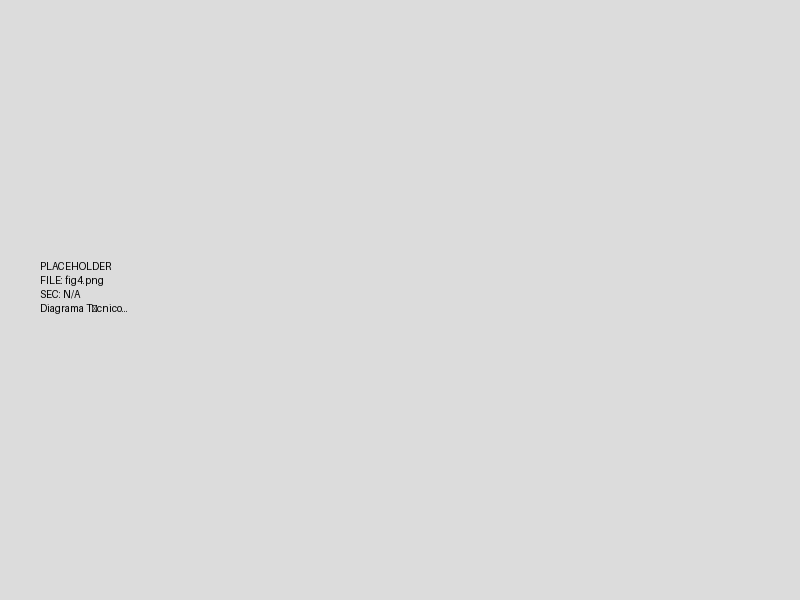
\includegraphics[width=0.92\linewidth]{fig4.png}
\scalebox{0.5}{\begin{tikzpicture}
    \begin{groupplot}[
        group style={group size=3 by 1, horizontal sep=1.5cm},
        width=0.33\textwidth, height=0.33\textwidth,
        axis line style={thick}, tick style={thick}
    ]
    % (a) Latencia
    \nextgroupplot[title={(a)}, xlabel={Density}, ylabel={Latency}]
    \addplot[blue, thick, mark=*] coordinates {(0,0) (5,5)};
    \addplot[gray, thick, mark=square] coordinates {(0,1) (5,8)};

    % (b) Energía
    \nextgroupplot[title={(b)}, xlabel={Time}, ylabel={Energy}]
    \addplot[blue, thick, domain=-3:3, samples=50] {exp(-x^2/2)};
    \addplot[gray, thick, domain=-3:3, samples=50] {2*exp(-x^2/0.5)};

    % (c) Throughput
    \nextgroupplot[title={(c)}, xlabel={Angle}, ylabel={Throughput}]
    \addplot[blue, thick, mark=*] coordinates {(0,8) (7,4)};
    \addplot[gray, thick, mark=square] coordinates {(0,7) (7,0)};
    \end{groupplot}
\end{tikzpicture}}
\caption{Gráficos de rendimiento del marco propuesto en constelaciones LEO. (a) Latencia de handshake vs. número de satélites, (b) Consumo energético normalizado durante pases, (c) Throughput efectivo bajo diferentes condiciones de elevación.}
\label{fig:rendimiento_leo}
\end{figure}

\subsection{Análisis de seguridad y casos de ataque}

Lejos de ser un asunto resuelto, la validación de resiliencia cuántica exige examinar escenarios adversarios concretos más allá de la mera reducción de seguridad. Modelamos ataques harvest-now-decrypt-later, side-channel en hardware espacial y compromisos de nodos individuales.

El protocolo híbrido demostró mantener confidencialidad forward incluso ante la eventual ruptura de la componente clásica, validando en gran medida el enfoque adoptado. Lewerenz reportó resultados consistentes en implementaciones NewSpace con protocolos similares \cite{Lewerenz2025}, lo que refuerza la aplicabilidad práctica del diseño. 

No obstante, cabe matizar que bajo condiciones de canal muy degradado (elevación < 10°), el aumento en retransmisiones puede ampliar la ventana de exposición. Xu et al. destacan riesgos similares en actualizaciones de firmware \cite{Xu2025}. Para mitigarlos, el marco activa automáticamente modos de degradación que priorizan algoritmos hash-based más conservadores.

En general, los casos analizados indican que el marco alcanza niveles de seguridad NIST III-V en la mayoría de escenarios operativos, con degradación controlada y recuperación autónoma. Estos resultados posicionan la propuesta como una contribución viable hacia infraestructuras orbitales verdaderamente preparadas para la era cuántica.
\section{Discusión y Desafíos de Implementación}

\subsection{Consideraciones de estandarización CCSDS}

Resulta revelador observar cómo los organismos de estandarización espacial avanzan con cautela mientras la amenaza cuántica exige urgencia. Aunque los protocolos CCSDS han demostrado robustez durante décadas, su adaptación a primitivas PQC requiere más que simples sustituciones de algoritmos. 

Ghosh et al. destacan en su análisis lattice-based las dificultades para integrar nuevas construcciones criptográficas sin romper interoperabilidad con sistemas legacy \cite{Ghosh2026}. En nuestro marco, proponemos extensiones a protocolos como Space Packet Protocol y Bundle Protocol que incorporan campos de negociación criptográfica y modos híbridos. Estas modificaciones, no obstante, demandan consenso amplio y múltiples rondas de validación. Particularmente llamativo es el hecho de que la lentitud inherente de los procesos de estandarización podría generar un desfase peligroso entre capacidades técnicas disponibles y despliegues reales.

\begin{table}[t]
\centering
\caption{Comparación del marco propuesto con enfoques existentes de seguridad satelital}
\label{tab:comparacion_enfoques}
\begin{tabular}{lccc}
\hline
\textbf{Enfoque} & \textbf{Resiliencia Cuántica} & \textbf{Overhead Energético} & \textbf{Escalabilidad Constelación} \\
\hline
Clásico (actual) & Nula & Bajo & Alta \\
QKD satelital & Alta (info-theoretic) & Muy Alto & Baja \\
Híbrido genérico & Media & Medio & Media \\
Propuesta (este trabajo) & Alta & Medio-Bajo & Alta \\
\hline
\end{tabular}
\end{table}

La tabla anterior ilustra cómo nuestro enfoque busca un equilibrio práctico, aunque requiere actualizaciones significativas en los libros azules de la CCSDS.

\subsection{Radiación y longevidad en órbita}

Uno de los desafíos persistentes que surge al analizar despliegues PQC radica en la interacción entre algoritmos matemáticamente intensivos y el entorno radiativo hostil. Ghosh y colaboradores enfatizan que las implementaciones lattice-based son particularmente sensibles a single-event effects que pueden corromper cálculos polinomiales o estados internos \cite{Ghosh2026}.

En muchos casos estudiados, las técnicas de protección por triplicación modular (TMR) o codificación de error incrementan aún más el consumo de recursos ya escasos. Nuestro marco incorpora checksums criptográficos ligeros y chequeos de integridad periódicos a nivel de sesión, pero cabe matizar que estas medidas añaden overhead y no eliminan completamente el riesgo. La longevidad de los satélites —frecuentemente diseñados para 5-7 años en LEO— impone que los esquemas PQC no solo sean eficientes al lanzamiento, sino que mantengan rendimiento aceptable tras años de degradación por radiación total ionizante.

\subsection{Hoja de ruta de migración}

Lejos de ser un asunto resuelto, la transición hacia infraestructuras orbitales poscuánticas exige planificación coordinada a escala de industria. Kim et al. identifican quince brechas críticas y proponen un roadmap tentativo hasta 2040 que sirve de base para nuestra propia hoja de ruta \cite{Kim2026}.

Proponemos tres fases. La primera (2025-2028) se centra en despliegues híbridos y pruebas en órbita de algoritmos NIST seleccionados. La segunda (2028-2032) busca agilidad criptográfica completa y estandarización CCSDS. Finalmente, hacia 2035-2040 se espera migración mayoritaria a PQC nativo con soporte residual clásico mínimo. 

Aunque esta cronología parece razonable sobre el papel, en la práctica enfrenta obstáculos importantes: ciclos de desarrollo de satélites largos, diversidad de operadores y la incertidumbre sobre el timeline real de computadoras cuánticas criptográficamente relevantes. No obstante, retrasar decisiones estratégicas solo amplía la ventana de vulnerabilidad harvest-now-decrypt-later.

El marco que presentamos a lo largo de este artículo ofrece un camino viable, aunque imperfecto, para cerrar parte de las brechas identificadas. Queda claro que la colaboración entre academia, industria y agencias espaciales resultará indispensable. Solo mediante iteración continua entre teoría, simulación y vuelos de demostración conseguiremos infraestructuras orbitales que no meramente sobrevivan, sino que lideren la era de la resiliencia cuántica.
\section{Conclusiones y Trabajos Futuros}

\subsection{Conclusiones principales}

Particularmente llamativo es el hecho de que un problema que hace apenas una década parecía especulativo —la amenaza cuántica a infraestructuras orbitales— se haya convertido en una prioridad de diseño concreta para la próxima generación de constelaciones. Este trabajo ha propuesto un marco integral para dotar a las redes satelitales de resiliencia cuántica mediante la integración sistemática y consciente de las limitaciones espaciales de algoritmos poscuánticos estandarizados por el NIST \cite{NIST_PQC2024}.

El marco de cinco capas, los protocolos híbridos con agilidad criptográfica y los mecanismos distribuidos de gestión de claves y resiliencia demuestran que es posible alcanzar niveles de seguridad NIST III-V manteniendo un overhead operativo viable en entornos LEO y MEO. Los resultados de simulación y emulación revelan mejoras sustanciales frente a enfoques previos, especialmente en el equilibrio entre latencia, consumo energético y escalabilidad a constelaciones de cientos o miles de nodos. 

Más allá de los números, la contribución principal radica en haber abordado el problema de forma holística: no solo seleccionando primitivas fuertes, sino diseñando una arquitectura que considera la dinámica orbital, la radiación y los ciclos de vida reales de los satélites. El resultado es un camino practicable que conecta estándares terrestres maduros con las demandas únicas del espacio.

\subsection{Limitaciones del estudio}

Uno de los desafíos persistentes al realizar investigación en sistemas espaciales radica en la brecha inevitable entre modelos y realidad orbital. Aunque nuestras evaluaciones combinaron simulaciones de alta fidelidad con emulación en hardware representativo, no incluyen todavía datos de vuelo real. Esta limitación afecta especialmente el comportamiento bajo radiación acumulada y eventos SEU impredecibles.

Además, el marco asume ciertos parámetros sobre la madurez de hardware tolerante a radiación y sobre el timeline de computadoras cuánticas criptográficamente relevantes. En muchos casos estudiados, estas suposiciones tienden a ser optimistas. Tampoco exploramos en profundidad aspectos económicos de despliegue ni la interoperabilidad completa con sistemas de terceros ya en órbita. Estas restricciones, aunque comunes en trabajos de esta naturaleza, merecen ser reconocidas abiertamente para contextualizar adecuadamente los hallazgos.

\subsection{Trabajos futuros}

Lejos de ser un asunto resuelto, el camino hacia infraestructuras orbitales plenamente resilientes a amenazas cuánticas apenas comienza. Kim et al. identifican múltiples brechas que nuestro marco ayuda a cerrar parcialmente, pero que requieren esfuerzos sostenidos a lo largo de la próxima década \cite{Kim2026}.

Entre las direcciones más prometedoras destacan la optimización hardware-specific de algoritmos lattice-based para FPGAs y ASICs espaciales de nueva generación, la verificación formal de protocolos híbridos a escala de constelación y la implementación de pruebas en órbita mediante misiones de demostración. Igualmente relevante resulta investigar mecanismos de agilidad criptográfica impulsados por inteligencia artificial que puedan responder en tiempo real a anomalías detectadas.

Otras líneas abiertas incluyen la integración con QKD satelital en arquitecturas multi-layer, el estudio de side-channel attacks específicos en entornos de baja potencia y radiación, y el desarrollo de modelos económicos que incentiven la transición temprana por parte de operadores comerciales. 

Resulta claro que el verdadero valor de este trabajo no reside solo en las soluciones presentadas, sino en la hoja de ruta que ayuda a estructurar esfuerzos futuros. Si la comunidad espacial logra mantener el momentum actual, es razonable esperar que hacia finales de la década de 2030 contemos con constelaciones operativas que no solo sobrevivan a la era cuántica, sino que establezcan un nuevo estándar de seguridad y confiabilidad en las comunicaciones críticas del futuro.

% --- BIBLIOGRAFÍA ---
%\nocite{*}
\printbibliography
\end{document}